% Template for submission of abstracts to NetSci 2025, Maastricht, the Netherlands.
% Modified from previous NetSci templates (NetSci2017, NetSci2016, STATPHYS25).
% The editors reserve the right to modify your submission.

% To compile, run with LaTeX2e

% ******** DO NOT EDIT ****************
\documentclass[10pt]{article}
% \usepackage{mathptmx}
\usepackage[margin=20mm]{geometry}
\usepackage{graphicx}
\usepackage{lmodern}
\usepackage{hyperref}
\usepackage{xcolor}
\usepackage{amsmath,amssymb}
\usepackage{titlesec}
\usepackage{sidecap}
% \usepackage{unsecrefs}
%\usepackage[letterpaper,margin=25.4mm]{geometry} % 1 inch margin
\usepackage[labelfont=bf]{caption}
%\usepackage{comment}
% \usepackage{natbib}  % Add this line for BibTeX support
\renewcommand{\familydefault}{\sfdefault}
%\pagestyle{empty}
%\setlength{\parskip}{0.25\baselineskip}
%\renewcommand{\title}[1]{{\noindent\large\bfseries#1\medskip\\}}
%\renewcommand{\author}[2]{{\noindent #1 \medskip\\ \noindent \small #2 \medskip}}
%\renewcommand{\vec}[1]{\boldsymbol{#1}}
%\def\vec#1{{\bm #1}}
%\def\tnull{{\text{null}}}
%\def\vec#1{{\bm #1}}
%\def\diag{\text{diag}}
%\def\mat#1{\mathbf{#1}}
%\def\Xmat{{\bm X}}
%\def\Exp{{\mathbb E}}
%\def\Var{\text{Var}}
%\def\ErdosRenyi{{Erd\H{o}s-R\'{e}nyi}\xspace}
%\def\given{\mid}
% Remove the section title for References
\renewcommand{\refname}{}

%%
\def\pin{p_\text{in}}
\def\pout{p_\text{out}}
\def\cin{c_\text{in}}
\def\cout{c_\text{out}}
\def\cave{\langle k \rangle}
\def\ECSstd{S_{\text{EC}}^{\text{std}}}
\def\ECS{S_{\text{EC}}}
\def\set#1{\mathcal{#1}}
\newcommand*\diff{\mathop{}\!\mathrm{d}}

% abbreviations
\def\eg{e.g.,~}
\def\ie{i.e.,~}
\def\cf{cf.\ }
\def\viz{viz.\ }
\def\vs{vs.\ }

%\renewcommand{\familydefault}{\sfdefault}
%\pagestyle{empty}
%\setlength{\parskip}{0.25\baselineskip}
\renewcommand{\title}[1]{{\noindent\large\bfseries#1\medskip\\}}
%\renewcommand{\author}[2]{{\noindent #1 \medskip\\ \noindent \small #2 \medskip\\}}
% *************************************

\begin{document}

% ********** USER DEFINED *************


% Enter title here
\title{Detectability threshold in weighted modular networks}
\noindent
{\footnotesize
Filippo Radicchi$^1$, Filipi N. Silva$^1$, Alessandro Flammini$^1$, Santo Fortunato$^1$, Sadamori Kojaku$^2$;
$^1$Center for Complex Networks and Systems Research, Luddy School of Informatics, Computing, and Engineering, Indiana University, Bloomington, IN, USA;
$^2$School of Systems Science and Industrial Engineering, Binghamton University, Binghamton, NY, USA
\par}

Community detection algorithms identify mesoscopic modular structure in networks by partitioning nodes into clusters with denser within-community connections than cross-community edges.
A fundamental question is: what is the maximum level of mixing between communities that still permits detection better than random guessing?
This detectability threshold has been extensively studied for unweighted networks using the planted-partition model (PPM), where communities become undetectable when the difference between within- and cross-cluster degrees falls below a critical value.
However, despite widespread application of community detection to weighted networks, the detectability threshold for weighted modular networks has remained unexplored.

We derive the detectability threshold for weighted networks using spectral modularity optimization on a weighted PPM with two equally sized communities.
Our analysis reveals a general expression showing that the threshold depends on the first two moments of both node degree and edge weight distributions.
Counterintuitively, we find that edge weights can \emph{undermine} community detection when they do not correlate with community structure---incorporating such weights narrows the detectable regime compared to ignoring them entirely.

We focus on networks with Poisson-distributed node degrees and compare five edge-weight distributions: Dirac (constant weights), Poisson, exponential, geometric, and signed Bernoulli.
We examine two complementary scenarios for how community structure manifests in weighted networks.
In the \emph{topology-based} case, communities are encoded through network structure---nodes have more edges to nodes in the same community ($\langle k_{\text{in}} \rangle > \langle k_{\text{out}} \rangle$) while edge weights are uniform across all connections.
In the \emph{weight-based} case, the network topology is homogeneous ($\langle k_{\text{in}} \rangle = \langle k_{\text{out}} \rangle$), but communities are encoded by assigning larger weights to within-community edges ($\langle w_{\text{in}} \rangle > \langle w_{\text{out}} \rangle$).

Our results reveal a hierarchy of detectability thresholds that holds across both scenarios (Figure).
Dirac weights yield the smallest (optimal) threshold, matching the unweighted PPM limit.
Exponentially distributed weights consistently increase the threshold by a factor of $\sqrt{2}$.
Poisson and signed-Bernoulli distributions exhibit variable behavior: they produce the largest thresholds for small total weights but approach the Dirac case as total weights increase.
Geometric weights show intermediate behavior, approaching the exponential case as total weights increase.
Critically, in the weight-based case, higher weight variance increases detectability thresholds, meaning more variable weights make communities harder to detect.
We validate these predictions using the Leiden algorithm on multi-community networks, confirming the same hierarchy across different numbers of communities.
Our results provide fundamental limits for community detection in weighted networks and guidance for when edge weights should be incorporated into detection algorithms.


\begin{figure*}[!htb]
    \centering
    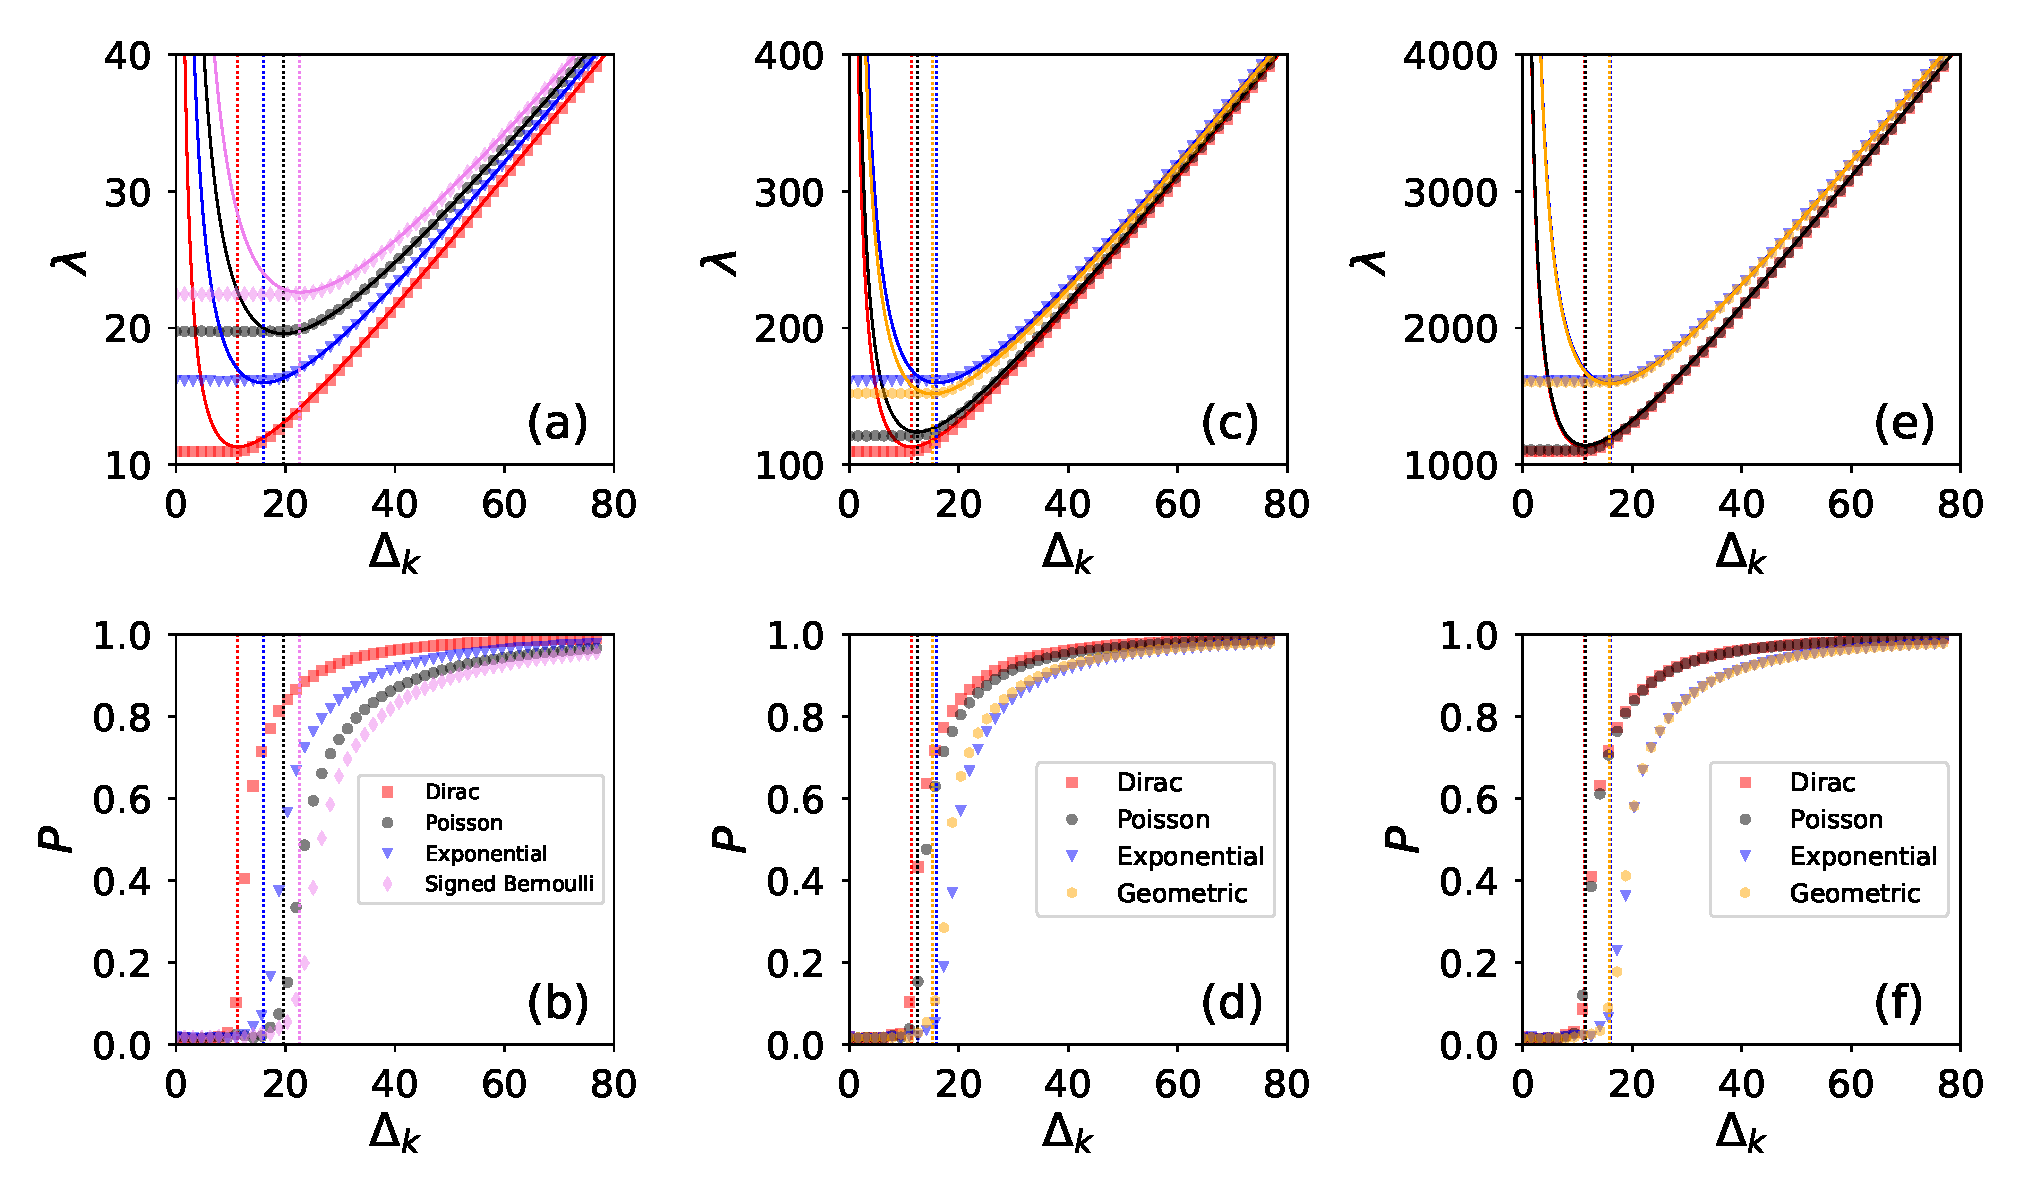
\includegraphics[width=0.7\textwidth]{../../figs/figure2.pdf}
    \caption{
        \textbf{Numerical validation of detectability thresholds.}
        Largest eigenvalue $\lambda$ of the modularity matrix as a function of difference between the expected value of the within- and cross-community degrees $\Delta_k$ for the weighted planted-partition model ($N=1024$, $K=128$, $W=1$).
        Different symbols/colors correspond to different edge-weight distributions.
        The transition from undetectable ($P\simeq 0$) to detectable ($P > 0$) regimes validates our theoretical predictions for the detectability hierarchy across weight distributions.
    }
    \label{fig:eigenvalue}
\end{figure*}

%\vspace{-5em}
%\bibliographystyle{unsrt}
%\bibliography{../../bibliography}

% *************************************
\end{document}

